\newpage
\section{Uložení workflow}
\nocite{demel:book}

K uložení nového modulu slouží tlačítko $Save$ ve spodní části postranního panelu. Nejdříve  zkontroluje, zdali graf (workflow) neobsahuje cyklus. Je-li graf v pořádku, otevře se dialogové okno pro nastavení informací o novém modulu. Z obrázku [\figurename \ref{wf:saveDialog}] je vidět, že uživatel zadává jméno modulu, tagy, popis a hlavně parametry. U nich se uživatel rozhodne, zdali je chce v novém modulu zadávat anebo se nebudou měnit a tudíž si nastaví jejich hodnotu při tvorbě modulu a nebude je zaškrtávat. U parametrů, které se budou měnit, uživatel zaškrtne zaškrtávací pole. Případně může zadat alternativní název parametru, který se mu bude zobrazovat místo stávajícího.

\begin{figure}[h]
	\centering
	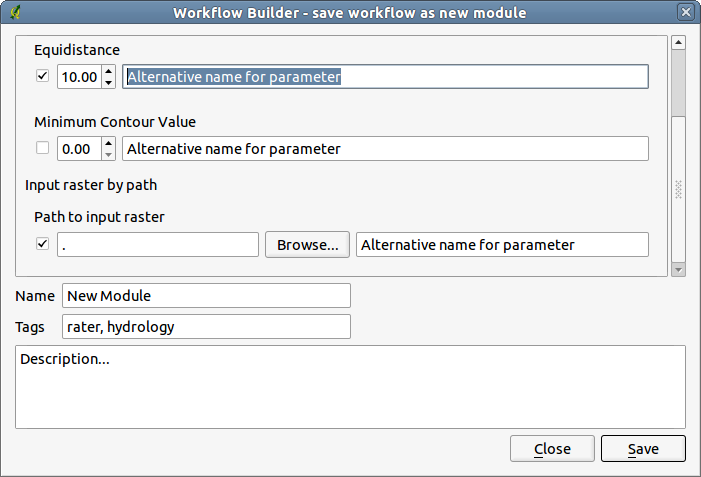
\includegraphics[scale=0.6]{pictures/wf/wf_saveDialog}
	\caption{Workflow Builder - dialog pro uložení nového modulu}
  	\label{wf:saveDialog}
\end{figure}

Po nastavení se klikne na tlačítko $Save$. Kontroluje se, zdali je zadán název nového modulu. Nový modul se uloží jako soubor ve formátu xml do \textbf{\$$HOME/.qgis/python/workflows$} s názvem stejným jako název modulu.  

\subsection{Výstupní xml souboru}
XML nabízí jednoduché uložení hierarchicky strukturovaných dat. O prvcích XML dokumentu hovoříme jako o elementech. Elementy jsou ohraničeny počátečními a koncovými značkami, tzv. tagy. XML dokument obsahuje vždy právě jeden kořenový element, který se může skládat z dalších a dalších elementů. V našem případě je kořenový element Graph. Ten se skládá z minimálně jednoho podgrafu (SubGraph) a ten poté minimálně z jednoho modulu (Module). Podgraf dále může obsahovat spojení mezi moduly (Connection). Modul kromě toho obsahuje elementy parametr (Port) a tag (tag) a také popis.  Tagy a popis jsou také obsaženy v Grafu. \\

\begin{table}[h]
	\centering
	\begin{tabular}{|c|c|}
		\hline
		atribut & příklad \\
		\hline
		name & Addition two rasters \\
		tags & ['raster', 'hydrology'] \\	
		\hline	
	\end{tabular}
	\caption{Atributy elementu Graph}
	\label{tab:graph}
\end{table}

Atributy elementu více méně korespondují s atributy objektů z Workflow Builderu. DOM reprezentace konkrétního parametru vypadá takto [\lstlistingname \ref{portDOM}].

\begin{lstlisting}[label=portDOM,caption={příklad DOM reprezentace parametru},morekeywords={Port}]
	<Port connected="True" default_value="[]" id="944" moduleID="897"
		  name="Raster" optional="False" porttype="1" should_be_set="False" 
		  type="processing.parameters.RasterLayerParameter" value="[]">
\end{lstlisting}